\documentclass[a4paper,12pt]{article}
\usepackage[utf8]{inputenc}
\usepackage{geometry}
\usepackage{fontspec}
\usepackage[scheme=plain]{ctex} % 提供中文支持及zihao命令
\usepackage{caption}
\captionsetup[figure]{labelformat=empty}
\usepackage{tikz}
\usepackage{float}
\usepackage{listings}
\usepackage{xcolor}
\usepackage{titlesec}
\usepackage{fancyhdr}
\usepackage{graphicx}
\usepackage{hyperref}

% 页面设置
\geometry{left=2.5cm, right=2.5cm, top=2.0cm, bottom=2.0cm}
\linespread{1.5}

% 字体设置 (请根据系统安装字体调整,这里使用常用字体)
% \setmainfont{Times New Roman}
% \setCJKmainfont[AutoFakeBold=true]{SimSun} % 宋体
% \setCJKsansfont[AutoFakeBold=true]{SimHei} % 黑体

% 标题格式设置
\titleformat{\section}{\centering\zihao{2}\heiti}{}{0em}{}
\titleformat{\subsection}{\zihao{3}\heiti}{}{0em}{}
\titleformat{\subsubsection}{\zihao{4}\heiti}{}{0em}{}
\titleformat{\paragraph}[runin]{\indent\zihao{-4}\heiti}{}{0em}{}[:]

% 颜色定义
\definecolor{codegreen}{rgb}{0,0.6,0}
\definecolor{codegray}{rgb}{0.5,0.5,0.5}
\definecolor{codepurple}{rgb}{0.58,0,0.82}
\definecolor{backcolour}{rgb}{0.95,0.95,0.92}

% 代码块设置
\lstdefinestyle{mystyle}{
    backgroundcolor=\color{backcolour},   
    commentstyle=\color{codegreen},
    keywordstyle=\color{magenta},
    numberstyle=\tiny\color{codegray},
    stringstyle=\color{codepurple},
    basicstyle=\ttfamily\footnotesize,
    breakatwhitespace=false,         
    breaklines=true,                 
    captionpos=b,                    
    keepspaces=true,                 
    numbers=left,                    
    numbersep=5pt,                  
    showspaces=false,                
    showstringspaces=false,
    showtabs=false,                  
    tabsize=2
}
\lstset{style=mystyle}

% 页眉页脚
\pagestyle{fancy}
\fancyhf{}
\fancyfoot[C]{\zihao{-5}\songti \thepage}
\renewcommand{\headrulewidth}{0pt}

% TikZ设置
\usetikzlibrary{shapes.geometric, arrows, positioning, shadows}

\begin{document}

% --- 封面或标题 ---
\begin{center}
    \vspace*{2cm}
    {\zihao{-0}\heiti 西北工业大学《移动应用开发》大作业报告} \\
    \vspace{4cm}
    
    {\zihao{3}\songti
    \begin{tabular}{rl}
        \textbf{题目:} & \textbf{西工大校园行} \\
        \textbf{} & \\
        \textbf{姓名:} & 王彦淞\quad 郭知宇 \\
        \textbf{学号:} & 2024303596\quad 2024303627 \\
        \textbf{班级:} & RB032401 \quad 14032409 \\
        \textbf{指导教师:} & 周果清 \\
        \textbf{提交日期:} & 2026年2月5日 \\
    \end{tabular}
    }
\end{center}

\newpage

% --- 正文 ---

\section{正文部分}

\subsection{1. 选题依据}

大学校园占地面积广阔,建筑分布复杂,对于新生、访客以及日常跨校区活动的师生而言,快速准确地定位目的地(如教学楼、宿舍、甚至具体的运动场入口)往往面临诸多不便。虽然市面上已有高德、百度等通用地图应用,但它们对于校园内部道路、特定建筑物名称索引以及校园专属设施(如特定实验室位置)的覆盖往往不够详尽,且无法提供针对校园场景的个性化服务。

本项目旨在基于华为 HarmonyOS 平台,利用 ArkTS 和 ArkUI 框架,开发一款轻量级、高性能的校园地图导航应用。通过直接解析 OpenStreetMap (OSM) 矢量数据,实现校园地图的自定义渲染与路径规划。该项目不仅具有很强的现实应用价值,能极大便利校园生活,同时也是对移动应用开发课程中 UI 绘制、数据解析、算法应用及系统能力调用的一次综合性实践与创新。

\subsection{2. 设计思路}

\subsubsection{2.1 整体架构}

本应用采用了典型的 MVVM (Model-View-ViewModel) 架构思想,并结合 HarmonyOS 的特性进行了模块化设计。整体架构分为三层:数据层 (Data Layer)、服务层 (Service Layer) 和 UI 展示层 (UI Layer)。

\begin{figure}[H]
\centering
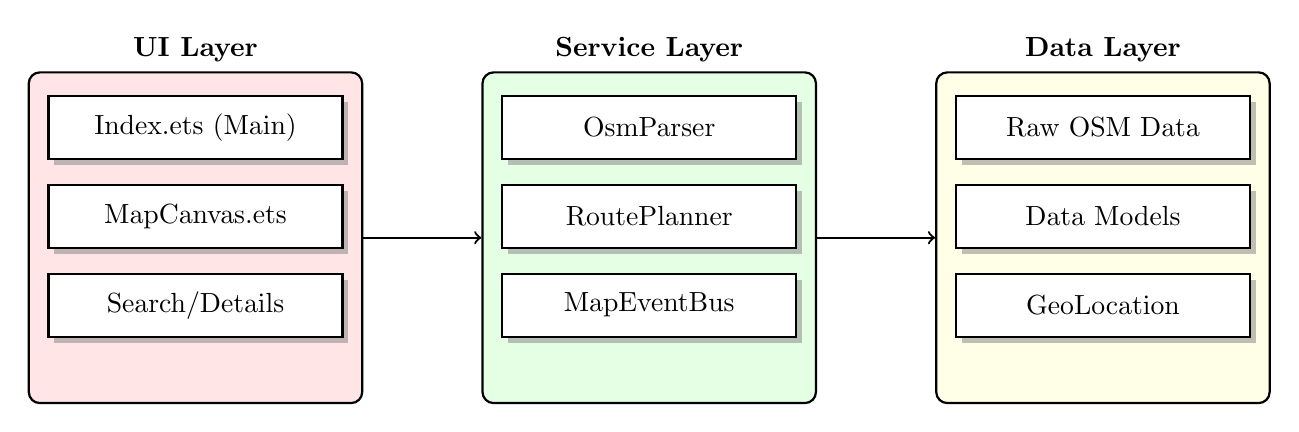
\begin{tikzpicture}[
    node distance=0.5cm,
    layer/.style={rectangle, draw=black, thick, fill=blue!10, text width=4cm, align=center, minimum height=4.2cm, rounded corners},
    module/.style={rectangle, draw=black, thick, fill=white, text width=3.5cm, align=center, minimum height=0.8cm, drop shadow}
]

    % UI Layer (Left)
    \node (ui) [layer, fill=red!10] {};
    \node [above] at (ui.north) {\textbf{UI Layer}};
    
    \node (index) [module, below=0.3cm of ui.north] {Index.ets (Main)};
    \node (canvas) [module, below=0.3cm of index] {MapCanvas.ets};
    \node (comps) [module, below=0.3cm of canvas] {Search/Details};

    % Service Layer (Middle)
    \node (service) [layer, fill=green!10, right=1.5cm of ui] {};
    \node [above] at (service.north) {\textbf{Service Layer}};
    
    \node (parser) [module, below=0.3cm of service.north] {OsmParser};
    \node (router) [module, below=0.3cm of parser] {RoutePlanner};
    \node (bus) [module, below=0.3cm of router] {MapEventBus};

    % Data Layer (Right)
    \node (data) [layer, fill=yellow!10, right=1.5cm of service] {};
    \node [above] at (data.north) {\textbf{Data Layer}};
    
    \node (osm) [module, below=0.3cm of data.north] {Raw OSM Data};
    \node (model) [module, below=0.3cm of osm] {Data Models};
    \node (sensor) [module, below=0.3cm of model] {GeoLocation};

    % Arrows
    \draw[->, thick] (ui) -- (service);
    \draw[->, thick] (service) -- (data);

\end{tikzpicture}
\caption{图1 系统整体架构图}
\end{figure}

\subsubsection{2.2 核心功能模块设计}

\begin{itemize}
    \item \textbf{OSM 数据解析模块} (`OsmParser.ets`):核心的数据处理引擎。不依赖第三方地图 SDK,而是直接读取 `.osm` (XML 格式) 地图文件。通过正则表达式流式处理 XML 节点,提取 `node` (坐标点) 和 `way` (路径/区域),识别 `highway` (道路)、`building` (建筑)、`natural` (水体) 等标签,构建内存中的矢量地理数据 `RenderData`。
    \item \textbf{地图渲染模块} (`MapCanvas.ets`):基于 Canvas API 的自定义渲染引擎。负责将经纬度坐标 (`LatLon`) 投影映射到屏幕平面坐标。实现了多图层绘制机制,依次绘制地基区域、水体、草地、建筑物、道路网和导航路径。支持深色模式 (Night Mode) 的动态配色切换。
    \item \textbf{路径规划模块} (`RoutePlanner.ets`):实现了基于地理信息的导航算法。首先将复杂的地理路径网络抽象为无向加权图 (Undirected Weighted Graph),由于校园内部道路网络相对稀疏,采用欧几里得距离作为权重,使用 Dijkstra 算法计算两点间的最短路径,并支持平滑渲染。
    \item \textbf{交互控制模块} (`MapEventBus.ets`):为了解决复杂的地图手势冲突,设计了事件总线机制,统一处理平移 (Pan)、缩放 (Pinch) 和点击 (Tap) 事件,并计算坐标变换矩阵。
\end{itemize}

\subsubsection{2.3 关键类设计}

为了清晰展示各模块之间的静态结构与依赖关系,下图详细描述了系统的类结构。其中 \texttt{Index} 作为控制层,协调 \texttt{OsmParser} 进行数据解析,并调用 \texttt{RoutePlanner} 计算路径,最终将数据传递给 \texttt{MapCanvas} 进行渲染。

\begin{figure}[H]
\centering
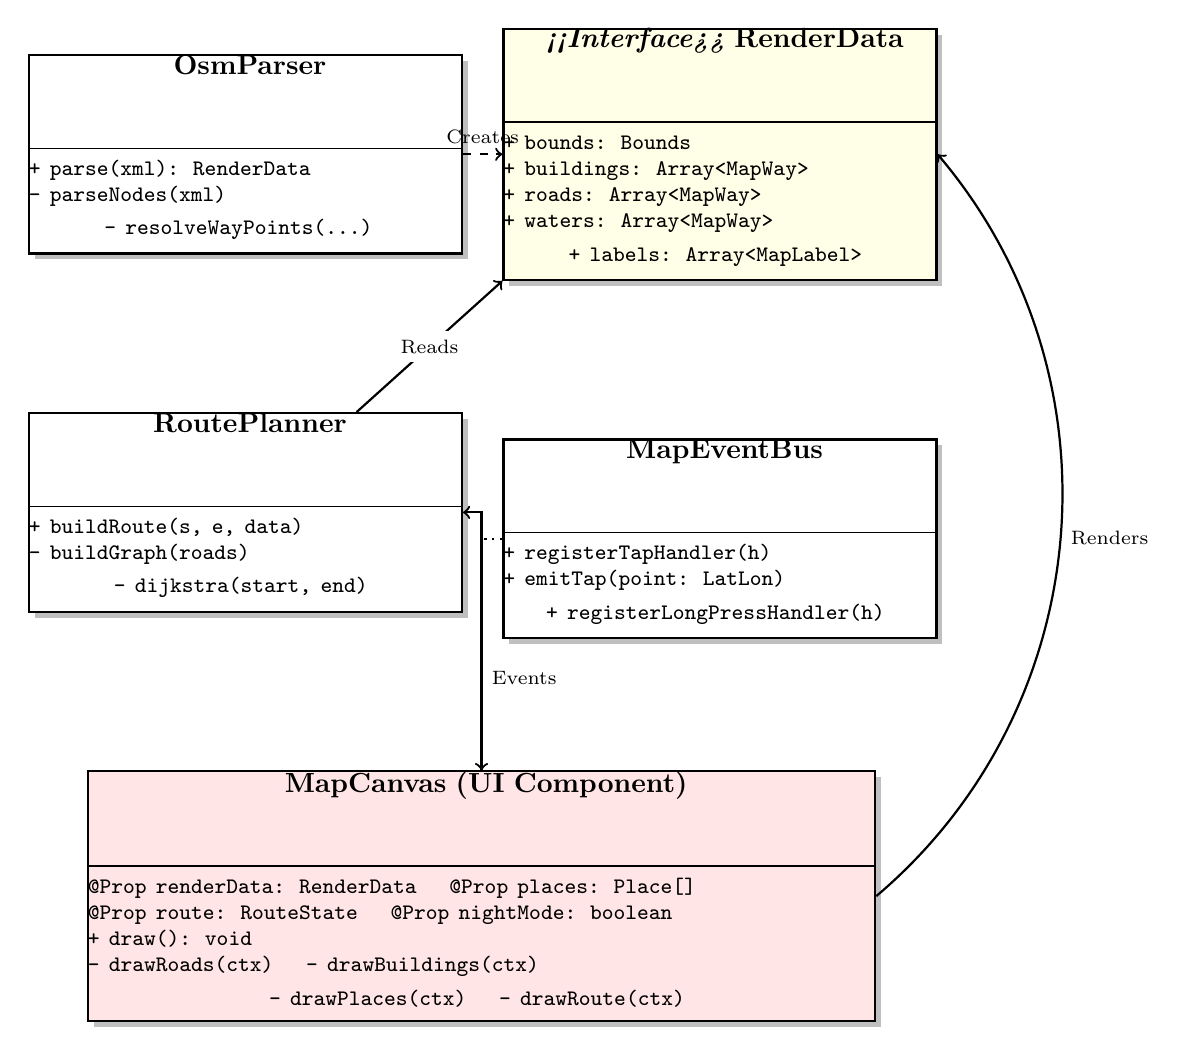
\begin{tikzpicture}[
    node distance=1.5cm,
    class/.style={
        rectangle,
        draw=black,
        thick,
        fill=white,
        drop shadow,
        text width=5.5cm,
        align=center,
        inner sep=0pt
    }
]

    % 1. OsmParser (Top Left)
    \node (parser) [class] {
        \vspace{15pt}
        \textbf{OsmParser} \\
        \rule{5.5cm}{0.5pt} \\
        \raggedright
        \footnotesize\ttfamily
        + parse(xml): RenderData \\
        - parseNodes(xml) \\
        - resolveWayPoints(...)
        \vspace{5pt}
    };

    % 2. RenderData (Top Right)
    \node (data) [class, fill=yellow!10, right=0.5cm of parser] {
        \vspace{15pt}
        \textbf{\textit{<<Interface>>} RenderData} \\
        \rule{5.5cm}{0.5pt} \\
        \raggedright
        \footnotesize\ttfamily
        + bounds: Bounds \\
        + buildings: Array<MapWay> \\
        + roads: Array<MapWay> \\
        + waters: Array<MapWay> \\
        + labels: Array<MapLabel>
        \vspace{5pt}
    };

    % 3. RoutePlanner (Middle Left)
    \node (planner) [class, below=2.0cm of parser] {
        \vspace{15pt}
        \textbf{RoutePlanner} \\
        \rule{5.5cm}{0.5pt} \\
        \raggedright
        \footnotesize\ttfamily
        + buildRoute(s, e, data) \\
        - buildGraph(roads) \\
        - dijkstra(start, end)
        \vspace{5pt}
    };
    
    % 4. MapEventBus (Middle Right)
    \node (bus) [class, below=2.0cm of data] {
        \vspace{15pt}
        \textbf{MapEventBus} \\
        \rule{5.5cm}{0.5pt} \\
        \raggedright
        \footnotesize\ttfamily
        + registerTapHandler(h) \\
        + emitTap(point: LatLon) \\
        + registerLongPressHandler(h)
        \vspace{5pt}
    };

    % 5. MapCanvas (Bottom)
    \node (canvas) [class, fill=red!10, below=2.0cm of planner, xshift=3cm, text width=10cm] {
        \vspace{15pt}
        \textbf{MapCanvas (UI Component)} \\
        \rule{10cm}{0.5pt} \\
        \raggedright
        \footnotesize\ttfamily
        @Prop renderData: RenderData \quad @Prop places: Place[] \\
        @Prop route: RouteState \quad @Prop nightMode: boolean \\
        + draw(): void \\
        - drawRoads(ctx) \quad - drawBuildings(ctx) \\
        - drawPlaces(ctx) \quad - drawRoute(ctx)
        \vspace{5pt}
    };

    % Relationships
    \draw[->, thick, dashed] (parser) -- node[above, font=\scriptsize] {Creates} (data);
    \draw[->, thick] (planner) -- node[font=\scriptsize, fill=white] {Reads} (data.south west);
    
    % Canvas dependencies
    \draw[->, thick] (canvas.north) |- (planner.east);
    \draw[<-, thick, dotted] (canvas.north) |- node[right, font=\scriptsize, pos=0.2] {Events} (bus.west);
    \draw[->, thick, bend right=45] (canvas.east) to node[right, font=\scriptsize] {Renders} (data.east);

\end{tikzpicture}
\caption{图3 核心模块类关系图}
\end{figure}

\subsection{3. 实现过程}

\subsubsection{3.1 数据预处理与解析}

项目首先解决了地图数据来源问题。通过导出校园区域的 OpenStreetMap 数据,在 `OsmParser.ets` 中利用正则匹配解析 XML 结构。

\begin{figure}[H]
\centering
\begin{tikzpicture}[node distance=2cm]
    \tikzstyle{startstop} = [rectangle, rounded corners, minimum width=3cm, minimum height=1cm,text centered, draw=black, fill=red!30]
    \tikzstyle{process} = [rectangle, minimum width=3cm, minimum height=1cm, text centered, draw=black, fill=orange!30]
    \tikzstyle{decision} = [diamond, minimum width=3cm, minimum height=1cm, text centered, draw=black, fill=green!30]
    \tikzstyle{arrow} = [thick,->,>=stealth]

    \node (start) [startstop] {开始解析};
    \node (read) [process, below of=start] {读取 .osm 文件};
    \node (nodes) [process, below of=read] {提取节点 (<node>)};
    \node (ways) [process, below of=nodes] {提取路径 (<way>)};
    
    \node (decide) [decision, right of=ways, xshift=4cm] {标签检查?};
    \node (build) [process, above of=decide, yshift=0.5cm] {建筑 / 区域};
    \node (road) [process, below of=decide, yshift=-0.5cm] {道路网络};
    
    \node (resolve) [process, right of=decide, xshift=4cm] {坐标解析与转换};
    \node (output) [startstop, below of=resolve, yshift=-0.5cm] {输出 RenderData};

    \draw [arrow] (start) -- (read);
    \draw [arrow] (read) -- (nodes);
    \draw [arrow] (nodes) -- (ways);
    \draw [arrow] (ways) -- (decide);
    \draw [arrow] (decide) -- node[anchor=east] {isBuilding} (build);
    \draw [arrow] (decide) -- node[anchor=east] {isHighway} (road);
    \draw [arrow] (build) -| (resolve);
    \draw [arrow] (road) -- (output.west);
    \draw [arrow] (resolve) -- (output);
\end{tikzpicture}
\caption{图2 OSM数据解析流程图}
\end{figure}

关键在于如何处理 `way` 中对 `node` 的引用。系统采用了 `Map<string, ParsedNode>` 结构来快速查找节点坐标,将抽象的引用 ID 转换为具体的经纬度序列,这是地图渲染的基础。

\subsubsection{3.2 地图渲染与坐标投影}

在 `MapCanvas.ets` 中,未采用简单的图片切片方案,而是实现了实时矢量绘制。核心难点在于经纬度到屏幕像素的转换。投影函数定义如下:

$$ x = \frac{(lon - minLon)}{lonSpan} \times width + offsetX $$
$$ y = \frac{(maxLat - lat)}{latSpan} \times height + offsetY $$

绘制时,`CanvasRenderingContext2D` 被大量使用。通过 `ctx.beginPath()`, `ctx.moveTo()`, `ctx.lineTo()` 勾勒出建筑轮廓和道路线条,并根据 `nightMode` 状态动态调整 `ctx.fillStyle` 和 `ctx.strokeStyle`,实现了日夜间模式的无缝切换。

具体的渲染流程如下图所示,系统依次加载数据、解析、校验,最终绘制到画布上。

\begin{figure}[H]
\centering
\begin{tikzpicture}[node distance=1.5cm]
    \tikzstyle{startstop} = [rectangle, rounded corners, minimum width=3cm, minimum height=1cm,text centered, draw=black, fill=red!10]
    \tikzstyle{process} = [rectangle, minimum width=3cm, minimum height=1cm, text centered, draw=black, fill=blue!10]
    \tikzstyle{decision} = [diamond, minimum width=2cm, minimum height=1cm, text centered, draw=black, fill=green!10, aspect=2]
    \tikzstyle{arrow} = [thick,->,>=stealth]

    \node (init) [startstop] {页面初始化};
    \node (read) [process, below of=init] {加载 map.osm};
    \node (parse) [process, below of=read] {OsmParser.parse()};
    \node (check) [decision, below of=parse] {解析成功?};
    \node (render) [process, below of=check, yshift=-0.5cm] {生成渲染数据};
    \node (draw) [process, below of=render] {MapCanvas.draw()};
    \node (display) [startstop, below of=draw] {地图显示};
    \node (error) [process, right of=check, xshift=3cm] {显示错误};

    \draw [arrow] (init) -- (read);
    \draw [arrow] (read) -- (parse);
    \draw [arrow] (parse) -- (check);
    \draw [arrow] (check) -- node[anchor=east] {是} (render);
    \draw [arrow] (check) -- node[anchor=south] {否} (error);
    \draw [arrow] (render) -- (draw);
    \draw [arrow] (draw) -- (display);
\end{tikzpicture}
\caption{图4 地图渲染管线}
\end{figure}

\subsubsection{3.3 路径规划算法实现}

导航功能在 `RoutePlanner.ets` 中实现。算法执行步骤如下:
\begin{enumerate}
    \item \textbf{图构建}:遍历所有解析出的道路数据 (`renderData.roads`),将所有道路交叉点和端点作为图的节点 (Node),道路线段作为边 (Edge),边的权重设为两点间的物理距离。
    \item \textbf{最近邻搜索}:当用户选择起点和终点时,首先遍历所有图节点,找到距离用户点击位置最近的道路节点作为算法的起终点。
    \item \textbf{Dijkstra 算法}:使用最小优先队列(或简单数组排序)维护开放列表,迭代计算从起点到所有可达节点的最短路径,直到访问到目标节点。
    \item \textbf{路径回溯}:从目标节点通过前驱指针列表回溯生成完整的坐标点序列,并在 MapCanvas 上以高亮线条绘制。
\end{enumerate}

下图展示了从用户交互到路径生成的完整逻辑闭环:

\begin{figure}[H]
\centering
\begin{tikzpicture}[node distance=1.5cm]
    \tikzstyle{startstop} = [rectangle, rounded corners, minimum width=3cm, minimum height=1cm,text centered, draw=black, fill=red!10]
    \tikzstyle{process} = [rectangle, minimum width=3cm, minimum height=1cm, text centered, draw=black, fill=blue!10]
    \tikzstyle{decision} = [diamond, minimum width=2cm, minimum height=1cm, text centered, draw=black, fill=green!10, aspect=2]
    \tikzstyle{arrow} = [thick,->,>=stealth]

    \node (start) [startstop] {用户点击};
    \node (handle) [process, below of=start] {MapEventBus 处理};
    \node (convert) [process, below of=handle] {屏幕坐标转经纬度};
    \node (node) [process, below of=convert] {寻找最近节点};
    \node (check) [decision, below of=node] {导航模式?};
    \node (planner) [process, right of=check, xshift=3.5cm, yshift=-1cm] {构建路径 (RoutePlanner)};
    \node (dijkstra) [process, below of=planner] {Dijkstra 算法};
    \node (overlay) [process, below of=dijkstra] {更新路径图层};
    \node (info) [process, below of=check, yshift=-1.5cm] {显示 POI 信息};

    \draw [arrow] (start) -- (handle);
    \draw [arrow] (handle) -- (convert);
    \draw [arrow] (convert) -- (node);
    \draw [arrow] (node) -- (check);
    \draw [arrow] (check) -| node[near start, above] {起终点已设} (planner);
    \draw [arrow] (check) -- node[anchor=east] {单击操作} (info);
    \draw [arrow] (planner) -- (dijkstra);
    \draw [arrow] (dijkstra) -- (overlay);
\end{tikzpicture}
\caption{图5 导航交互逻辑}
\end{figure}

\subsubsection{3.4 地点贡献与审核机制}

为了增强地图的互动性,应用支持用户长按地图添加新的地点信息。为了保证数据的准确性,系统内嵌了一套审核机制。用户提交的数据首先暂存至云端数据库,状态标记为“待审核”。管理员在后台审核通过后,该地点才会对所有用户可见。

\begin{figure}[H]
\centering
\begin{tikzpicture}[node distance=1.5cm]
    \tikzstyle{startstop} = [rectangle, rounded corners, minimum width=3cm, minimum height=1cm,text centered, draw=black, fill=red!10]
    \tikzstyle{process} = [rectangle, minimum width=3cm, minimum height=1cm, text centered, draw=black, fill=blue!10]
    \tikzstyle{decision} = [diamond, minimum width=2cm, minimum height=1cm, text centered, draw=black, fill=green!10, aspect=2]
    \tikzstyle{arrow} = [thick,->,>=stealth]

    \node (start) [startstop] {用户长按};
    \node (input) [process, below of=start] {输入信息};
    \node (submit) [process, below of=input] {提交申请};
    \node (check) [decision, below of=submit] {数据有效?};
    \node (db) [process, below of=check, yshift=-0.5cm] {保存至数据库 (待审)};
    \node (admin) [decision, below of=db, yshift=-0.5cm] {管理员批准?};
    \node (publish) [startstop, below of=admin, yshift=-0.5cm] {公开发布};
    \node (reject) [process, right of=admin, xshift=3cm] {通知驳回};

    \draw [arrow] (start) -- (input);
    \draw [arrow] (input) -- (submit);
    \draw [arrow] (submit) -- (check);
    \draw [arrow] (check) -- node[anchor=east] {是} (db);
    \draw [arrow] (check.east) -- ++(0.5,0) |- (input.east);
    \draw [arrow] (db) -- (admin);
    \draw [arrow] (admin) -- node[anchor=east] {是} (publish);
    \draw [arrow] (admin) -- node[anchor=south] {否} (reject);
\end{tikzpicture}
\caption{图6 地点贡献与审核流程}
\end{figure}

\subsection{4. 后端服务与 API 实现}

根据当前工作区根目录的 `server.ts` 实现,后端采用原生 `node:http` + `better-sqlite3` 的轻量架构,主要特性如下:

\begin{itemize}
    \item \textbf{技术栈与部署}:基于原生 HTTP(无 Express),SQLite WAL 模式持久化;邮件发送使用 126 SMTP(`nodemailer`),默认端口 8080,对外统一返回 JSON。
    \item \textbf{数据模型}:表涵盖 `users`(含 email、hiddenPlaceIds)、`places`、`feedback`、`tokens`、`system_overrides`、`messages`、`verification_codes`,启动时自动迁移,并支持从 `data/db.json` 导入旧数据。
    \item \textbf{鉴权与账户}:`/api/register`、`/api/login` 返回 Bearer Token 并写入 `tokens`;`/api/me` 基于 Token 返回当前用户;保留初始管理员账号 `admin/admin123`。
    \item \textbf{邮箱验证码闭环}:`/api/email/send` 生成验证码(purpose=`bind`/`reset`,5 分钟有效,存入 `verification_codes` 并发送邮件);`/api/email/bind` 校验后写入邮箱;`/api/password/reset` 校验验证码并更新密码,要求账户已绑定邮箱且邮箱匹配。
    \item \textbf{地点与审核 API}:`/api/places` 系列提供创建、更新、删除、提交审核 (`/publish`)、投票 (`/vote`)、反馈 (`/feedback`);管理员可通过 `/api/admin/places/:id/approve|reject` 审核 pending 记录;公共与个人视图通过 `scope=public|mine|pending` 获取。
    \item \textbf{系统覆盖与消息}:`/api/system-overrides` 提供系统级覆盖数据;`messages` 表记录审核/通知信息,随用户会话读取。
    \item \textbf{文件上传}:支持图片直传至 `data/uploads`,限制 10MB,校验 MIME/扩展名,外链路径 `/images/{id.ext}` 基于请求 Host 动态拼接。
\end{itemize}

整体 API 设计与 `server-api.md` 文档一致:注册/登录获取 Token;绑定邮箱后方可完成密码找回;地点提交先 pending,管理员审核通过后公开。

\subsection{5. 对课程的建议}
鸿蒙开发对于扩展学生的视野和技能有很大帮助,但是门槛相对较高,希望在课程中能够详细讲解开发全流程.
课程的作业安排相对单一,希望之后的作业布置能不局限于我的家乡小程序的逐步润色,通过更加丰富的作业设计
吸引同学们对移动应用开发的兴趣.我们总体对课程非常满意,感谢老师和助教的辛勤付出!
